\section{Thread}

\begin{frame}[fragile]{Thread: Light-Weight Process}
	\only<2>{
		\begin{figure}[H]
			\centering
			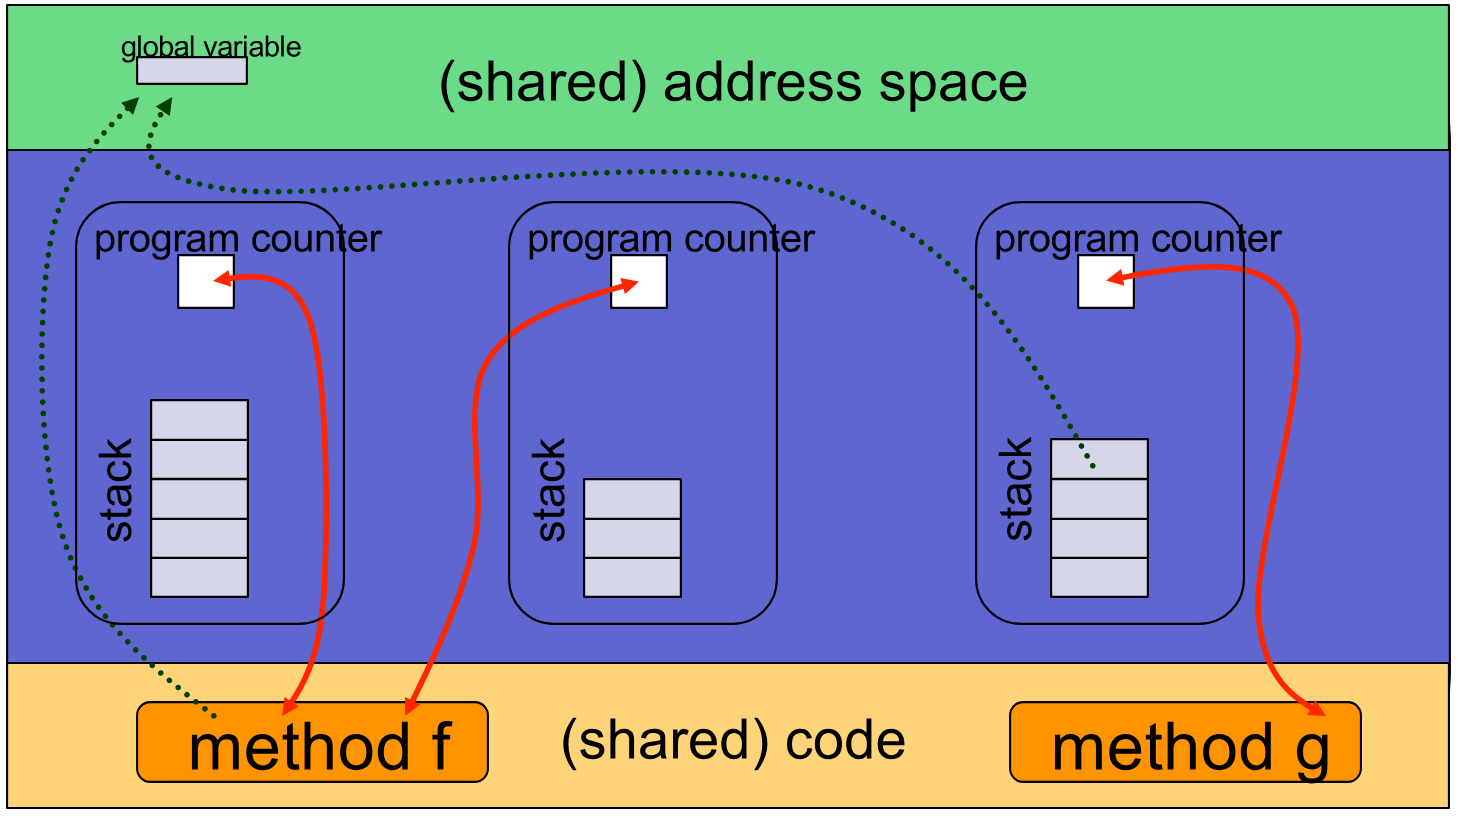
\includegraphics[width=0.8\textwidth]{day3/img/thread.png}
		\end{figure}
	}
	\only<1>{
		\begin{itemize}
			\item \emoji{star} A thread is a \textbf{basic unit of execution} within a process. Each thread has its own:
			      \begin{itemize}
				      \item Thread ID
				      \item Program counter
				      \item Register set
				      \item Stack
			      \end{itemize}
			\item Shares the following with other threads within the same process:
			      \begin{itemize}
				      \item Code section
				      \item Data section
				      \item The heap (dynamically allocated memory)
				      \item Open files and signals
			      \end{itemize}
			\item \textbf{Concurrency}: A multi-threaded process \textbf{can do multiple things at once}
		\end{itemize}
	}
\end{frame}

% \begin{frame}[fragile]{OpenMP: Multi-Thread in Practice}
% OpenMP
% \end{frame}
